\chapter{Materials and methods}
\label{Chap3}
Description expériences et machines
\section{Powder follow-up}

\subsection{Sieving}

\subsection{Grain size and distribution}

\subsection{Composition}

%\subsection{Drying}

\section{Process parameters}
The same direct metal printer (DMP) was used to fabricate all specimens throughout this work. It is a \textit{ProX DMP 200} printer, manufactured by \textit{3D Systems} (see figure \ref{fig:Printer}). It uses a laser with a theoretical maximal power of 300 [W] and wavelength $\lambda$ = 1070 [nm] \parencite{3D}. Its actual maximal power is $P_{max}=273.6$.  The maximal envelope capacity of the machine (W x D x H) is 140 x 140 x 125 [mm]. Its typical accuracy is +/- 50 [$\mu m$] for small parts and +/- 0.2\% for large parts. It allows for the set-up of a protection atmosphere. However, it does not integrate any heating feature for the build bed.\\

\begin{figure}[th]
\centering
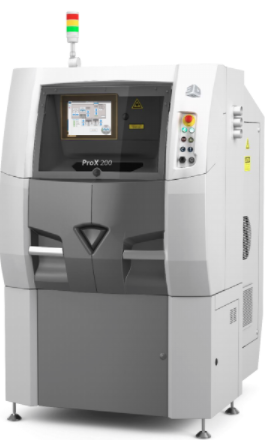
\includegraphics[scale=0.7]{Images/Printer}
\decoRule
\caption[ProX DMP 200 printer]{ProX DMP 200 printer (from the user's ProX DMP 200 general instructions document).}
\label{fig:Printer}
\end{figure}

In this thesis, argon was used as shielding gas. The composition of the gas environment was monitored so as to keep $p_{O2}$ < 1000 [ppm]. [Corrections, paramètres laser etc...]. Values for h and t were respectively set to 100 [$\mu m$] and 30 [$\mu m$]. The other process parameters were varied so as to optimize the properties of the built specimens. Educated guesses were made based on literature and previous works done at the UCL. The parameters used are resumed in table \ref{table:Pparam}. Batches were named in the format X200-\textit{yymmdd}. The prefix "X200" refers to the DMP used. It is followed by the date of printing (6 digits). Recycled powder was used for every batch except for X200-180222 and X200-180228. [Dual scan strategy] . Dimensions of the cubic and cylindrical specimens are noted in accordance with figure \ref{fig:cc}.\\

 %\begin{center}
\begin{table}[ht]
\noindent\makebox[\textwidth]{\begin{tabular}{|c|c|c |c |c|c|c|}

    \hline
  Batch name & Contour & Type & Dimensions [mm] &Specimen name & $\frac{P}{P_{max}} [-]$ & $v_s [\frac{mm}{s}]$\\
  \hline
  \hline
  X200-171024 & No & Cubic & L=10& 1 & 0.85 & 900\\
  & &   & & 2 &  & 1000\\
  & &   & & 3&  & 1059\\
  & &  & & 4&  & 1500\\
  & &  & & 5& 1 & 900\\
  & &  & & 6&  & 1059\\
  & & & & 7, 7a, 7b & 0.75 & 1200\\
  & & & & 8, 8a, 8b& & 900\\
\hline  
  X200-180109 & No&Cubic & L=10 & 7c,...7q (15 spec.)& 0.75 &1200\\
  & & & & 8c,...8q (15 spec.)  & & 900\\
\hline  
  X200-180220 & No & Cubic & L=5 & TT150-2 & 0.75 & 1200\\
  & &  & & TT200-2 &  &\\
  & &  & & TT300-2 &  &\\
  & &  & & TT300-2-plaque &  &\\
  & &  & & TT150-2-real &  &\\
  & &  & & TT200-2-real &  &\\
  & &  & & TT250-2-real &  &\\
  & &  & & TT300-2-real &  &\\
\hline  
  X200-180222 & No & Cubic & L=10 &12& 0.75 & 1200\\
  & &  & &13 &  &\\
\hline  
  X200-180228  & Yes & Cylindrical & D=6, H=2 &1 & 0.75 & 1200\\
  & &  &  & 2&  & \\
  & &  &  & 3 &  & \\
\hline  
  X200180313 & Yes & Cylindrical & D=6, H=10&1& 0.75 & 1200\\
    & &    & &2 & &  \\
    & &  &D=12, H=10 &3& &  \\
    & & & &4 & & \\
\hline  
  X200-180319  & Yes & Cubic & L=10 & cub 1 & 0.75 & 1200\\
  & &  & & cub 2 & &\\
  & &  & & cub 3 & &\\
  & & & & cub 4 & &\\
  & & & & cub 5 & &\\
  & & &  L=5& TT??????? &  &\\ 
  & &  Cylindrical & D=6, H=10&cyl 1   &  & \\
    & &  & &cyl 2 & & \\
    & &  & D=12, H=10 &cyl 3 & & \\
    & &  &  &cyl 4  & & \\

    \hline

\end{tabular}}
\caption[Process parameters used for the specimens manufacturing]{Process parameters used for the specimens manufacturing}
\label{table:Pparam}
\end{table}
 %\end{center}
 
\begin{figure}[th]
\centering
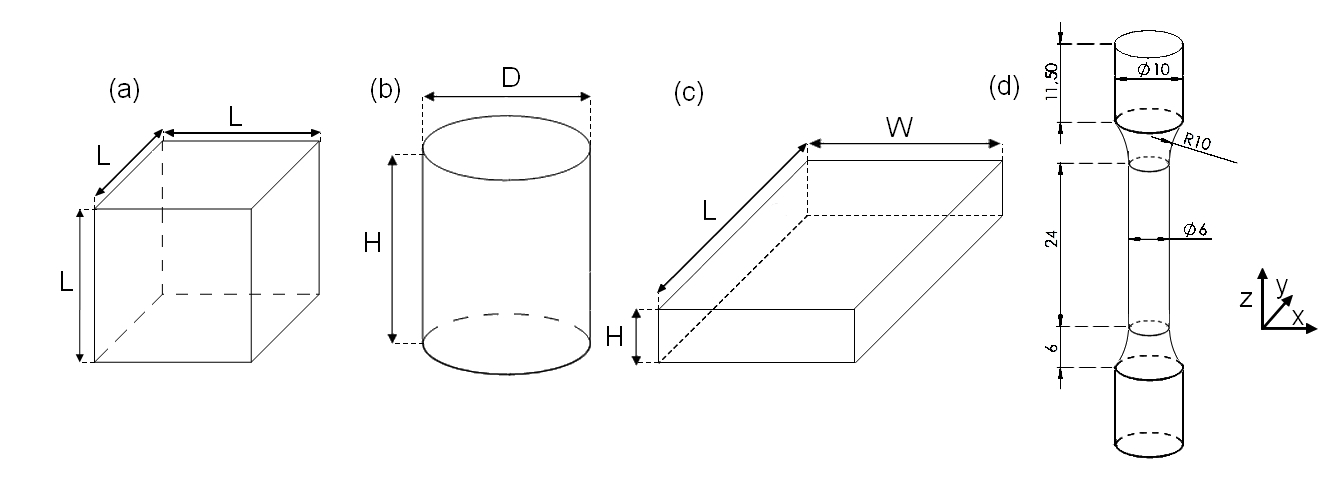
\includegraphics[scale=0.58]{Images/cc}
\caption[Dimensions notations for (a) cubic specimens (b) cylindrical specimens]{Dimensions notations for (a) cubic specimens (b) cylindrical specimens}
\label{fig:cc}
\end{figure}

Insérer images des positions d'échantillons. Aller chercher les ordres de fabrication

Caption des images Batch ... specimens position and order of fabrication

A hexagonal scanning strategy was chosen.. Pourquoi? On nous a pas vraiment demandé notre avis.

Insérer images de trajets du laser.

\section{Heat treatments}

The heat treatments were conducted inside a unique oven of the ... model, manufactured by ..., which is able to reach a temperature of 400\degree C. Samples temperature data was obtained through a thermocouple, welded to the sample surface. The data was displayed and saved every 10 seconds, with a precision of 0.1\degree C, thanks to a ..., connected to the thermocouple (see Fig. for both devices). \\

Samples that were subject to a heat treatment were named in a particular format, to ease distinction between them. They receive the name of the batch, followed by "TT-\textit{holdingtemperature-holdingtime-specific conditions}".

\section{Characterisation}

\subsection{Density}

\subsubsection{Hydrostatic weighing}

Multiple methods were considered to compute the apparent relative density of the fabricated specimens. The first one is hydrostatic weighting (also called hydrodensitometry). It is a direct application of the well-known Archimedes' principle, which can be stated as follows: " When a body is (partially or totally) immersed in a fluid, the upthrust on the body is equal to the weight of fluid displaced." \parencite{ADictionaryofPhysics}. By weighing each pieces in air and in water - giving respectively values of dry weight $W_a$ and underwater weight $W_w$ - one can estimate the apparent density $\rho_a$:

$$\rho_a=\frac{W_a}{W_a-W_w} \cdot \rho_w $$

where $\rho_w$ is the water density. The apparent relative density $\rho_{rel}$ of the specimens can then be calculated with:

$$\rho_{rel} = \frac{\rho_a}{\rho_b} $$

where $\rho_b = 2.68 [\frac{g}{mm^3}]$ is the theoretical bulk density of AlSi10Mg \parencite{Bulk}. All weightings were done with a \textit{Sartorius BP121S} analytical balance with precision of 0.1 [mg] \parencite{Balance}. Samples were immersed in demineralised water for more than twelve hours before the measurements to impregnate them. The weightings were also done in demineralised water. Water temperature was measured with a precision glass thermometer to compute $\rho_w$ as accurately as possible thanks to tabulated values \parencite{Eau}.\\

The technique was employed with both "as-built" and polished cubes, in order to mitigate possible air trapping by the surface roughness, that would distort the results. %to observe potential inhomogeneous distributions of the closed porosities in the specimens.
All six faces of the tested cubes were polished with P320 silicon carbide sandpaper sheets and briefly with P1200 ones.\\

\subsubsection{Image analysis}

In order to get as close as possible to the real relative density of the various samples, a third method to estimate it was used. Pictures of the polished sections of samples were taken under the optical microscope. With the help of the ImageJ software, the surface fraction occupied by porosities could be extracted. If we approximate that the surface fraction is equal to the volumetric one, we obtain an estimation of the relative density.

\subsection{Microscopy}

\subsubsection{Scanning electron microscope microscopy}

\subsubsection{Optical microscopy}

\subsection{Mechanical properties}

\subsubsection{Hardness test}

\subsubsection{Traction test}

\subsubsection{Fatigue}
